\documentclass[a4paper]{article}
\usepackage[utf8]{inputenc}
\usepackage[english, swedish]{babel}
\usepackage{amsmath}
\usepackage{graphicx}
\usepackage[colorinlistoftodos]{todonotes}
\usepackage{float}

\title{Lend and Lease}

\author{Group 3}

\begin{document}
\maketitle
\begin{center}

\includegraphics{logo.png}\\[1cm]
\begin{abstract}
A web application for leasing and borrowing items in your area.
\end{abstract}
\end{center}
\newpage
\tableofcontents
\newpage

\section{Motivation for our system}
Most people have valuable items lying around their home that they rarely or never use. The items might not serve a purpose for them daily, but they are still not something that they want to sell or get rid off. It’s for items like these that this website exists. 
With our website people can upload an image and input some information about the item and then lend or rent it out to people in their area. 

\section{Business Model}
The vision of what the site should be is rather simple: to let everyone that visits the site have access to the core of functionalities of the site. Allow them browse what items are available in their area without logging in. They should not have to navigate through the site to find out what it is they can do. It should all be there on the frontpage - a map with all the items in their area. From that map they can filter for items they’re interested in and then click on items of interest on the map and get the details of the item.

Our business plan with this would be to populate the site with users that like its simplicity and the fact that everything is handled between the two people involved in the renting or lending. When the user-base is sufficiently large we would start to advertise on the page. For example, when a user is looking at a screwdriver that he or she wants to borrow, there could be an ad for Amazon, showing the similar screwdrivers they have for sale, etc. 

We would also offer a premium membership for people that rent-out their things, allowing them to be featured on the site so that people can access their personal page and browse what items they offer. 

\section{System Function Specification}
\begin{itemize}
\item \textbf{Create Account} : This Function would allow users to Register themselves and start using the site.
\item \textbf{Log in \& Log out} 
\item \textbf{Forgot Password, send email to user} : In case user forgets their  login credentials, they should be able to reset it with a recovery email. 
\item \textbf{Adding new Items to lending-list} : Adding new Items that users want to lend to other people can be done with this "Add new Items" form.
\item \textbf{Adding requests for items} : Able to make requests for items.
\item \textbf{Send request for item to user} : Able to request items from the lender.
\item \textbf{Accept request send notification} : Send notification for the accepted requests.
\item \textbf{Filter Items by Categories} : Able to filter items by Categories.
\item \textbf{Search for items by name and categories} : Able to search items by its name and categories 
\item \textbf{Filter by Location} : Able to Filter the items by location.
\item \textbf{View Item Requests} : Able to view Item Requests
\item \textbf{View posted items} : Able to view all posted items.

\end{itemize}

\section{System Architecture }
\begin{figure}[H] 
  \centering
  \includegraphics[width=0.9\textwidth]{System_Architecture.png}\hfill
  \caption{System Architecture}\label{System Architecture}
\end{figure}


\section{Use Case } As previously mentioned our user-experience is built on the philosophy that a user should be able to access the core functionalities of the site without having to register and logging in. The user should get a good idea of what the site is about and what it offers before he or she is forced to register their email and come up with a password for the site. \\
For convenience, we have separated Use Case Diagram into two : \\ 
1) Users Interaction with Items \ref{UseCase-Items}  \\ 
2) User Registration and Profile \\

\subsection{User Interaction with Items}
\begin{itemize}
\item \textbf{Request Items} : Borrower should be able to send request for Items that he sees on the Item lists.
\item \textbf{Cancel Item Requests}: Borrower is able to cancel his past requests should he change his mind.
\item \textbf{Browse Items}: Able to browse different Items that are available.
\item \textbf{Search Items}: Able to search for a specific Item.
\item \textbf{Filter Available Items}: Able to filter items by location or type.
\item \textbf{Place an Item} : Lender is able to place items he wishes to lend.
\item \textbf{Accept Requests} : Lender is able to accept or decline the requests he receives.
\item \textbf{Put Items on Hold} : Lender can put an item on hold for which the Request will be on pending state on Borrowers end.
\item \textbf{View list of personal items} : Able to view list of all personal items that Lender has uploaded.
\item \textbf{Modify Existing items}: Able to modify details or specs for the Existing Items as necessary.
\end{itemize}

\begin{figure}[H] 
  \centering
  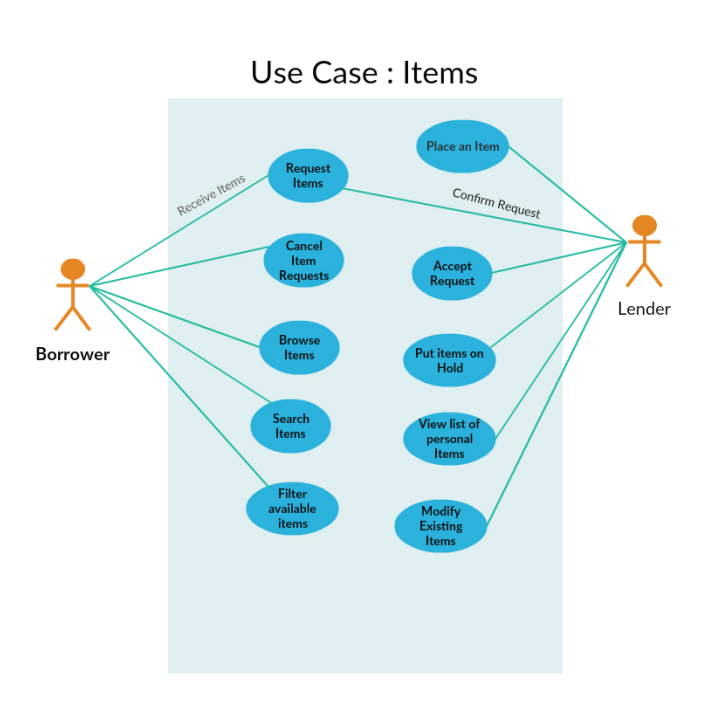
\includegraphics[width=0.9\textwidth]{usecase-Items.PNG}\hfill
  \caption{Users interaction with Items}\label{UseCase-Items}
\end{figure}

\subsection{User Registration \& Profile}
\begin{itemize}
\item \textbf{Sign up}: New User Registration
\item \textbf{Sign In} : Sign In for Existing Users
\item \textbf{View Notifications} : View Notifications regarding Item Requests.
\item \textbf{View Profile} : View one's profile.
\end{itemize}
\begin{figure}[H] 
  \centering
  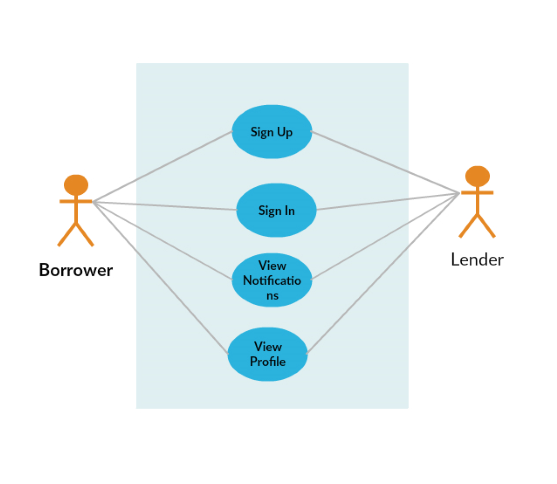
\includegraphics[width=0.9\textwidth]{usecase-Users.PNG}\hfill
  \caption{User Registration \& Profile}\label{Usecase-users}
\end{figure}



\section{ER model} All user-data item information is stored in our MySQL database. The main entities of our System are : User, Items and Requests as shown inside Red Rectangle block in ER Diagram \ref{ERDiagram}.  Associated attributes for each entities are shown in the ER Diagram within the blue spherical block. \\  We will briefly discuss their relationship and specialization. 
\begin{itemize}
\item \textbf{Relationship and specialization}: The type of relationship that can be seen in our system are: 
\begin{itemize}
\item \textbf{has a} : User and items have \textbf{has a} relationship and is one-to-many.
\item \textbf{is a} : User has \textbf{is a} relationship to show two types of users.The entity User is divided into two sub-group : Borrower and lender. This specialization can be seen in ER diagram as \textbf{IS A} relationship.
\item \textbf{creates} : user can create(borrower) or accept(lender) multiple requests. Therefore, the relationship between user and requests is one-to-many.
\end{itemize}

\end{itemize}
\begin{figure}[H] 
  \centering
  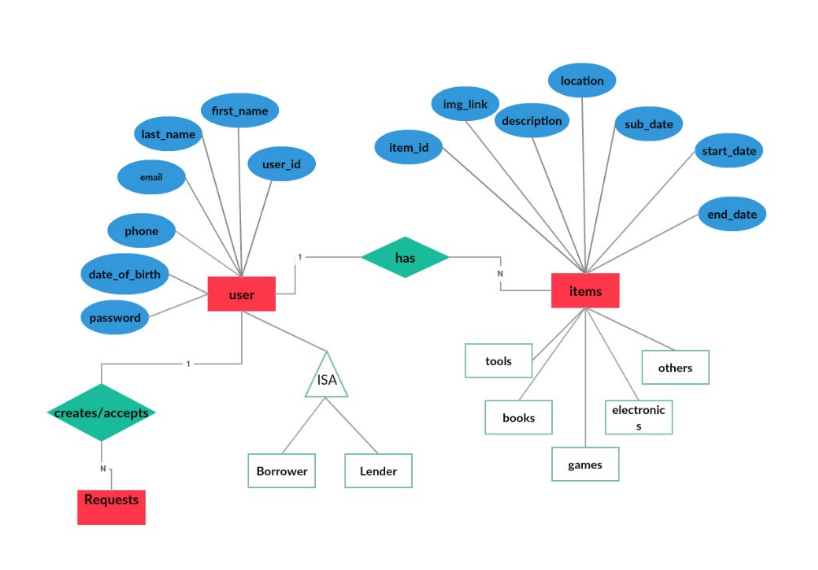
\includegraphics[width=0.9\textwidth]{ERfinal.PNG}\hfill
  \caption{ER Diagram}\label{ERDiagram}
\end{figure}

\section{System Implementation \& Evaluation}
\subsection{Implementation of functionality}
The functionalities we were able to implement were: 
\subsubsection{Add Items :} To be able to add items and specify its details such as name, category etc.
\begin{figure}[H] 
  \centering
  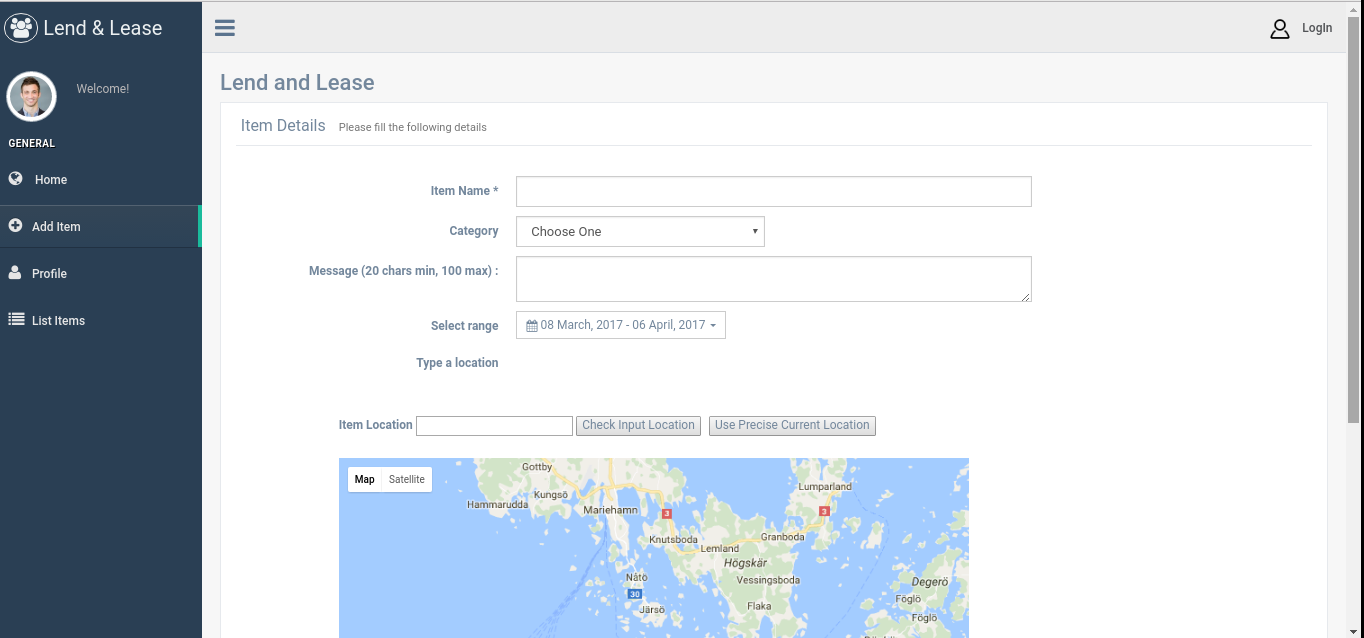
\includegraphics[width=0.9\textwidth]{addItems.PNG}\hfill
  \caption{Add items}\label{additems}
\end{figure}

\subsubsection{List Items :}  This functionality is there for users to be able to view items they are interested in. If they find anything they need/want in the list, they can make request for the items using the Request form.

\subsubsection{Profile :} To be able to view/ edit user's profile
\begin{figure}[H] 
  \centering
  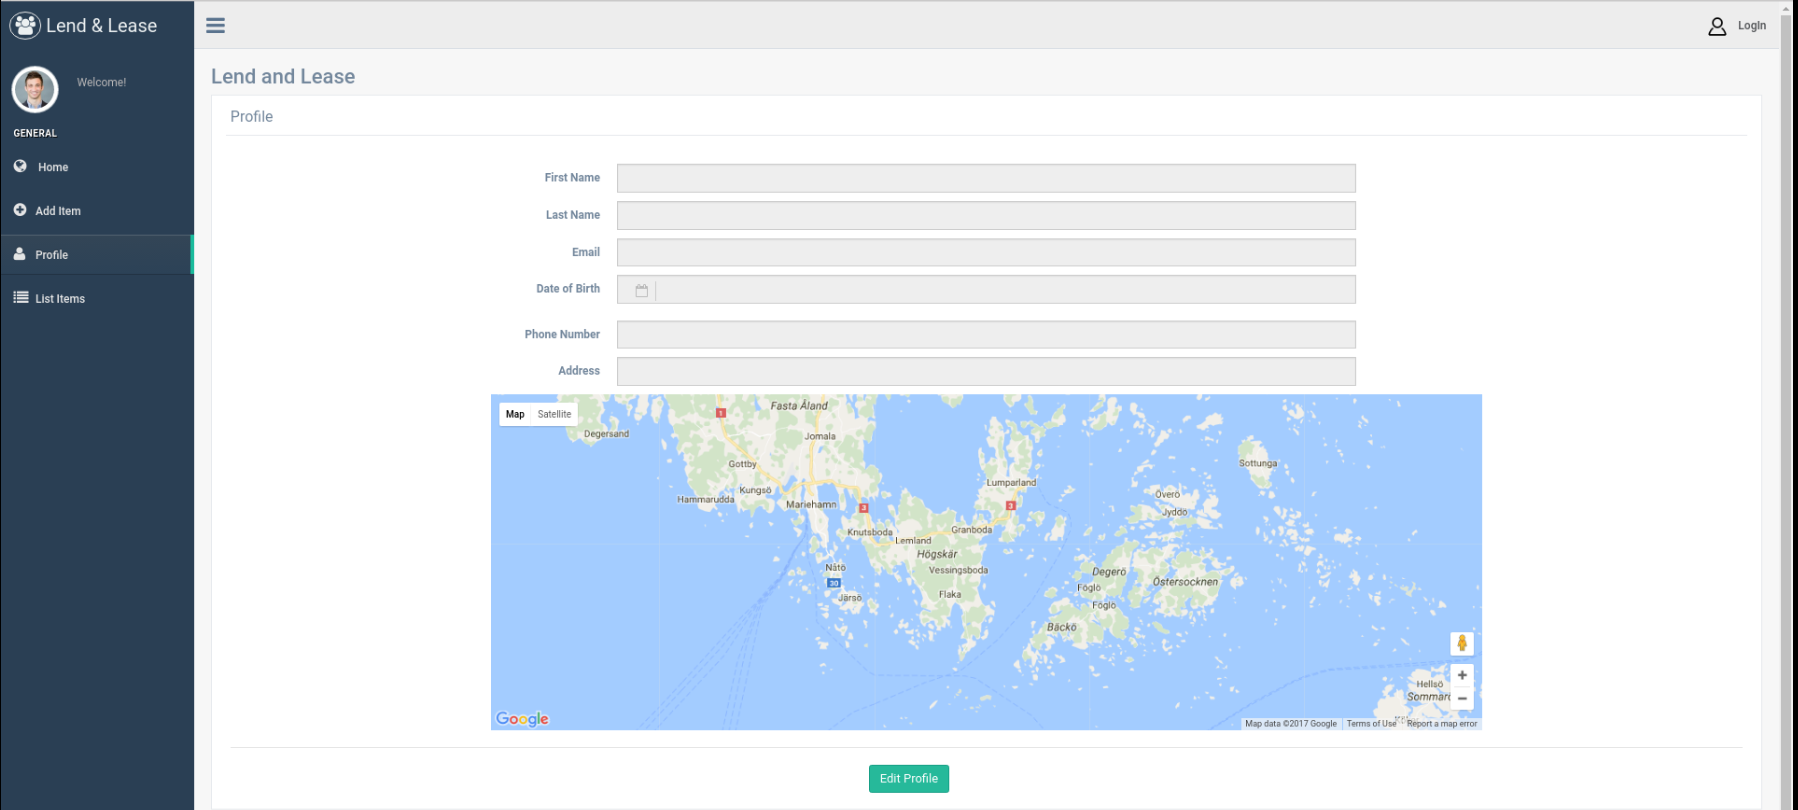
\includegraphics[width=0.9\textwidth]{profile.PNG}\hfill
  \caption{user Profile}\label{profile}
\end{figure}

\subsubsection{Maps :} Maps is available on the Home page as well as other pages. Using this, users can select the region they are interested in and starting browsing items filtered by location. 
\begin{figure}[H] 
  \centering
  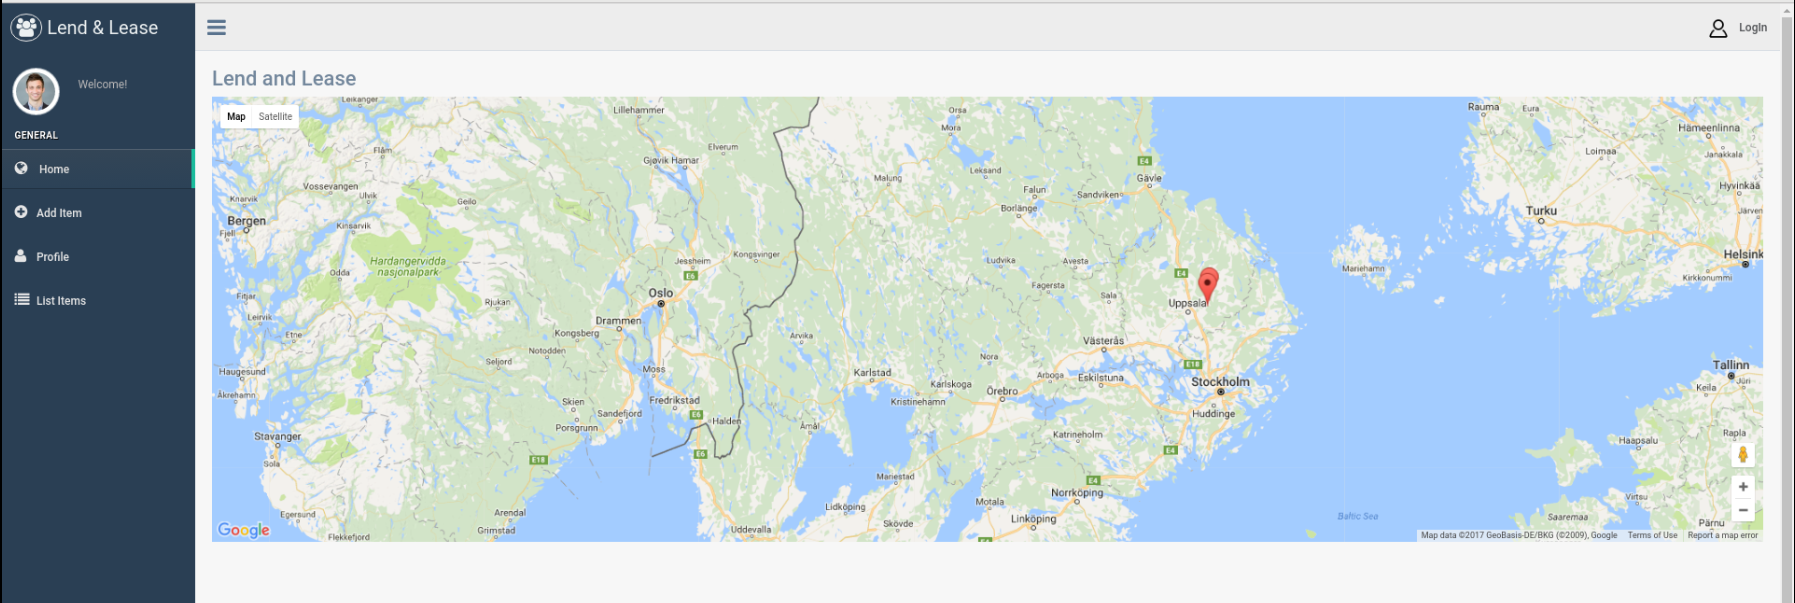
\includegraphics[width=0.9\textwidth]{home.PNG}\hfill
  \caption{Maps from Home page}\label{home}
\end{figure}
%screenshot

\subsection{Development Tools}
\begin{enumerate}
\item Github: For version control, we used Github to share code.
\item AngularJS : The Front-End of the system is using Google’s own framework - AngularJS. This is a perfect language for building dynamic web-applications and it fits perfectly with what we wanted our website to be. We wanted it to be a single-page application, with a sidebar for navigation and functionalities, leaving the center of the page to display information to the user and let him or her input their own information. 

\item NodeJS : The server built with NodeJS, using the express package to handle the HTTP requests and responses. What makes us satisfied with this choice is that NodeJS also has a package for communicating with MySQL databases which is our database of choice.

\item MySQL : For our database management we’re using MySQL. The reason being that it’s widely used and well-documented. Since AngularJS and NodeJS are somewhat new and poorly-documented we wanted something sturdy and trusted running the background if all else failed. 
\item node\_modules
\begin{itemize}
\item bcrypt-nodejs : used for encrypting user password. \cite{bcrypt}
\item express : used as a NodeJS web framework. \cite{express}
\item passport : used for Authentication. \cite{authentication}
\end{itemize}
\end{enumerate}

\section{Technical Problems Encountered } As we picked new languages and framework such as Angular, Node, it was difficult to get around with it. If we encountered some error, it was time consuming and annoying to find a fix for it. Also, there weren't good enough documentation available to get a quick overview. 

\section{Testing and Security}
\subsection{Testing} We have been doing testing on parallel along with development. It's a manual testing we're doing with no special testing framework used as of yet.

\subsection{Security}
\subsubsection{Password Encryption} we used native NodeJS library called bcrypt for encrypting and storing users password which uses the latest Security Recommendation for cryptographic algorithm. \cite{bcrypt} 

\subsubsection{Session Implementation} Establish login session for user and destroy it when logged out. 

\section{Group Management}
We initially started with everyone trying to learn the new language and familiarize with the frameworks we planned to use. As the time was closing by, we had to get started on the project and so we started dividing work as front end features and back end features.
As the project was running and after midterm presentation, we had to re-form the task division because not everyone was on the same pace and time was almost approaching deadline. So, the final work division was done as : two members on front-end, two on backend, and one on Report writing. 

\section{Future Work}
The feature that we initially planned to implement but were not able to because of limited time was : 
\subsection{Chat Functionality} We initially planned to implement Chat functionality in our App. This feature would enable requester and requestee to interact with each other and establish some kind of method to do the exchange of items they have.
\subsection{Testing} We didn't have time to do testing in an efficient and correct way. Given more time, we would have liked to implement some testing frameworks such as mocha which is a javascript test frameworks that runs on nodejs. Also, we would have liked to use some standard testing methods like: QAcomplete, HP QC etc and create test cases and run them properly in parallel with development.

\section{Conclusion} 
The implementation we have so far is what we plan to deploy. As mentioned earlier, the languages \& frameworks we used were new so it was a bit of annoyance to pick it up. Also, because of limited time, we had to throw away some features we initially planned to work on. 

\section{Source Code}
TBA

\begin{thebibliography}{}	  
    
    \bibitem{bcrypt}
    bcrypt-nodejs,  A native JS bcrypt library for NodeJS, [Online].\\
    Available: https://www.npmjs.com/package/bcrypt-nodejs
    
    \bibitem{authentication}
    Authentication, "Easy Node Authentication", [Online]. \\
    Available: https://scotch.io/tutorials/easy-node-authentication-setup-and-local
    
    \bibitem{express}
    Express, "Web Framework for NodeJS", [Online]. \\
    Available: http://expressjs.com/
    
\end{thebibliography}

\end{document}